\chapter{Case Study: Beam Response and Stain Gage}\label{c:strain}

In this chapter we will work through and example data acquisition design problem.  Our goal is present a complete system, with as much detail as possible, capable of measuring the response (static and dynamic) of a cantilevered beam subject to a load.

\section{Static Model: Cantilevered Beam}

Figure~\ref{f:cant} shows the solution to the classical beam equation for a cantilevered beam with a load placed at the tip.  This simple case illustrates how we can predict the moment ($M(x)$) and deflection ($y(x)$) in the structure as a function of the applied load.

\begin{figure}[hb!]
\centerline{
{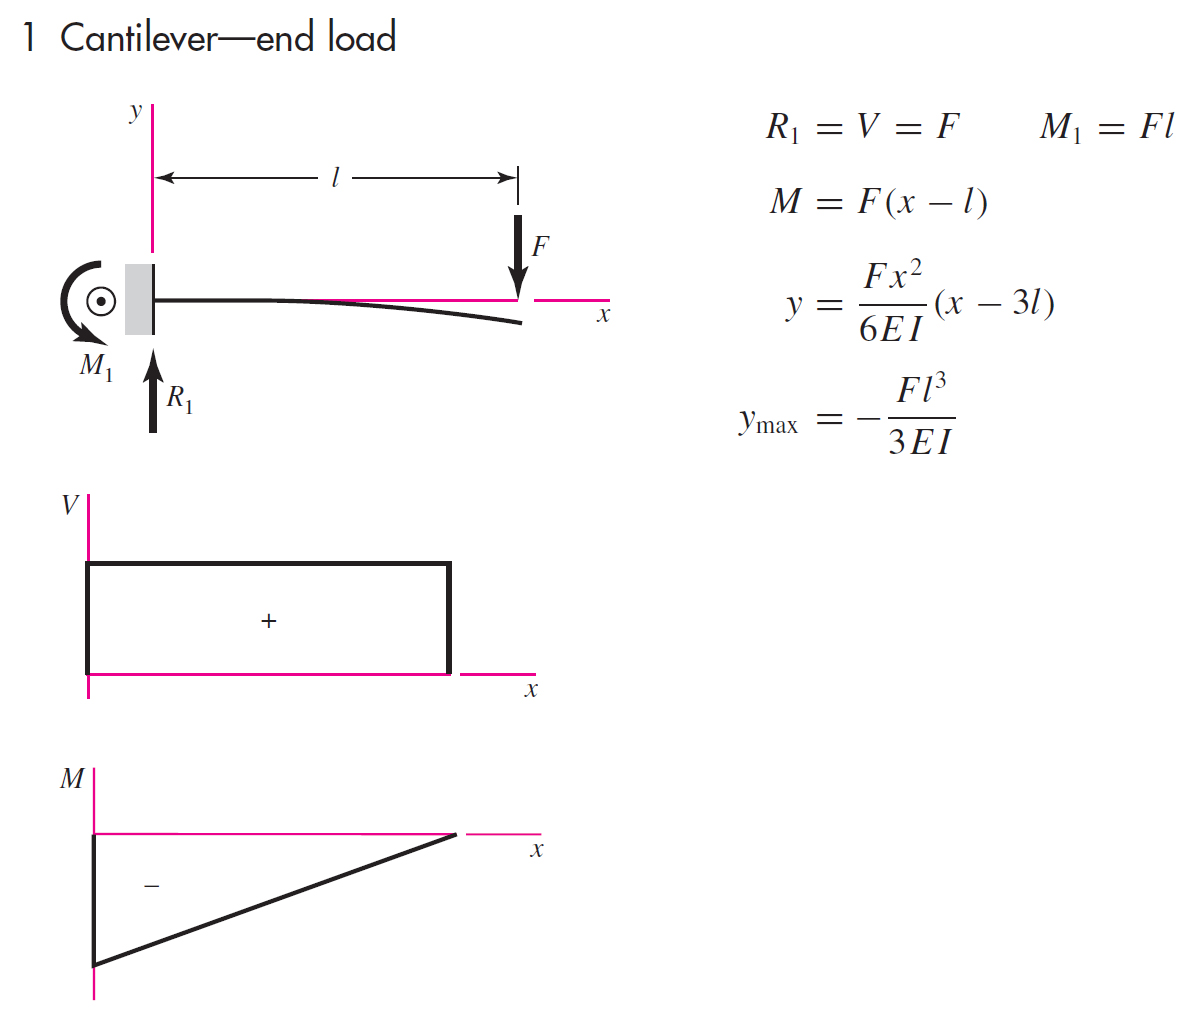
\includegraphics[width=0.5\textwidth]{cant_beam.jpg}}}
\caption{Shear, moment and deflection of a cantilevered beam.  Courtesy of \emph{Shigley's Mechanical Engineering Design}, 8th Edition, Budynas and Nisbett.}
\label{f:cant}
\end{figure}


\subsection{Determining Strain and Displacement}
Two quantities of the response of the beam that we'd like to be able to predict is the strain ($\epsilon$), due to bending, at a particular location along the length ($x$) as a function of the applied load ($F$) and the displacement at the free end of the beam ($y_{max}$) as a function of the applied load.  We can start with the (hopefully) familiar expression for bending stress in a beam due to an applied moment,
\[
\sigma_x=\frac{M(h/2)}{I},
\]
where $h$ is the height of the beam cross-section and $I$ is the second moment of area of the beam cross-section.  We can use the linear relationship for elastic stress and strain ($\sigma_x = E \epsilon$) to find an expression for the strain at any location $x$ along the beam:
\begin{equation}\label{e:eps}
\epsilon = \frac{F(x-l)(h/2)}{EI}.
\end{equation}
We can then solve for the tip force and the tip displacement as a function of the measured strain:
\begin{equation}\label{e:strainf}
F = \left( \frac{EI}{(x-l)(h/2)} \right) \epsilon 
\end{equation}
and
\begin{equation}\label{e:straine}
y_{max}=\left( \frac{l^3}{3(x-l)(h/2)} \right) \epsilon.
\end{equation}
These two equations are models of the response of a cantilevered beam. The first model (\ref{e:strainf}) predicts the force at the free end of the beam ($F$) as a function of the strain.  The second model (\ref{e:straine}) predicts the displacement at the free end of the beam as a function of the strain.

\section{Sensor: Strain Gage}
In our example we are going to use a stain gage to measure the deformation (strain) at one location in our bending beam.  Based on this estimate of deformation we can infer the strain and stress in the structure as well as the motion of the beam.  The sensor we will use is a \gls{strain gage} or more specifically, a bonded resistance strain gage.  This sensor, illustrated in Figure~\ref{f:strain} is a very common measurement tool for mechanical systems.  The type of strain gage we are considering is bonded to a surface so that when that element is deformed, the strain gage is deformed by the same amount.  This deformation causes the resistance of the foil grid (see Figure~\ref{f:strain}) to change according to the relationship
\begin{equation}\label{e:gage}
\mathrm{GF} = \frac{\delta R / R}{\delta L / L}=\frac{\delta R /R}{\epsilon}
\end{equation}
where $R$ is the nominal resistance of the strain gage (e.g., \unit[120]{Ohms}), $\delta R$ is the change in resistance, $L$ is the length of the gage, $\delta L$ is the change in length and $\epsilon$ is the strain at the location of the gage.  For metallic foil strain gages, GF is typically close to 2.  Since the stain in engineering devices is usually less than 1\%, which suggests that the change in resistance in a strain gage is very small, typically less than 1\%.  

\begin{figure}[hb!]
\centerline{
{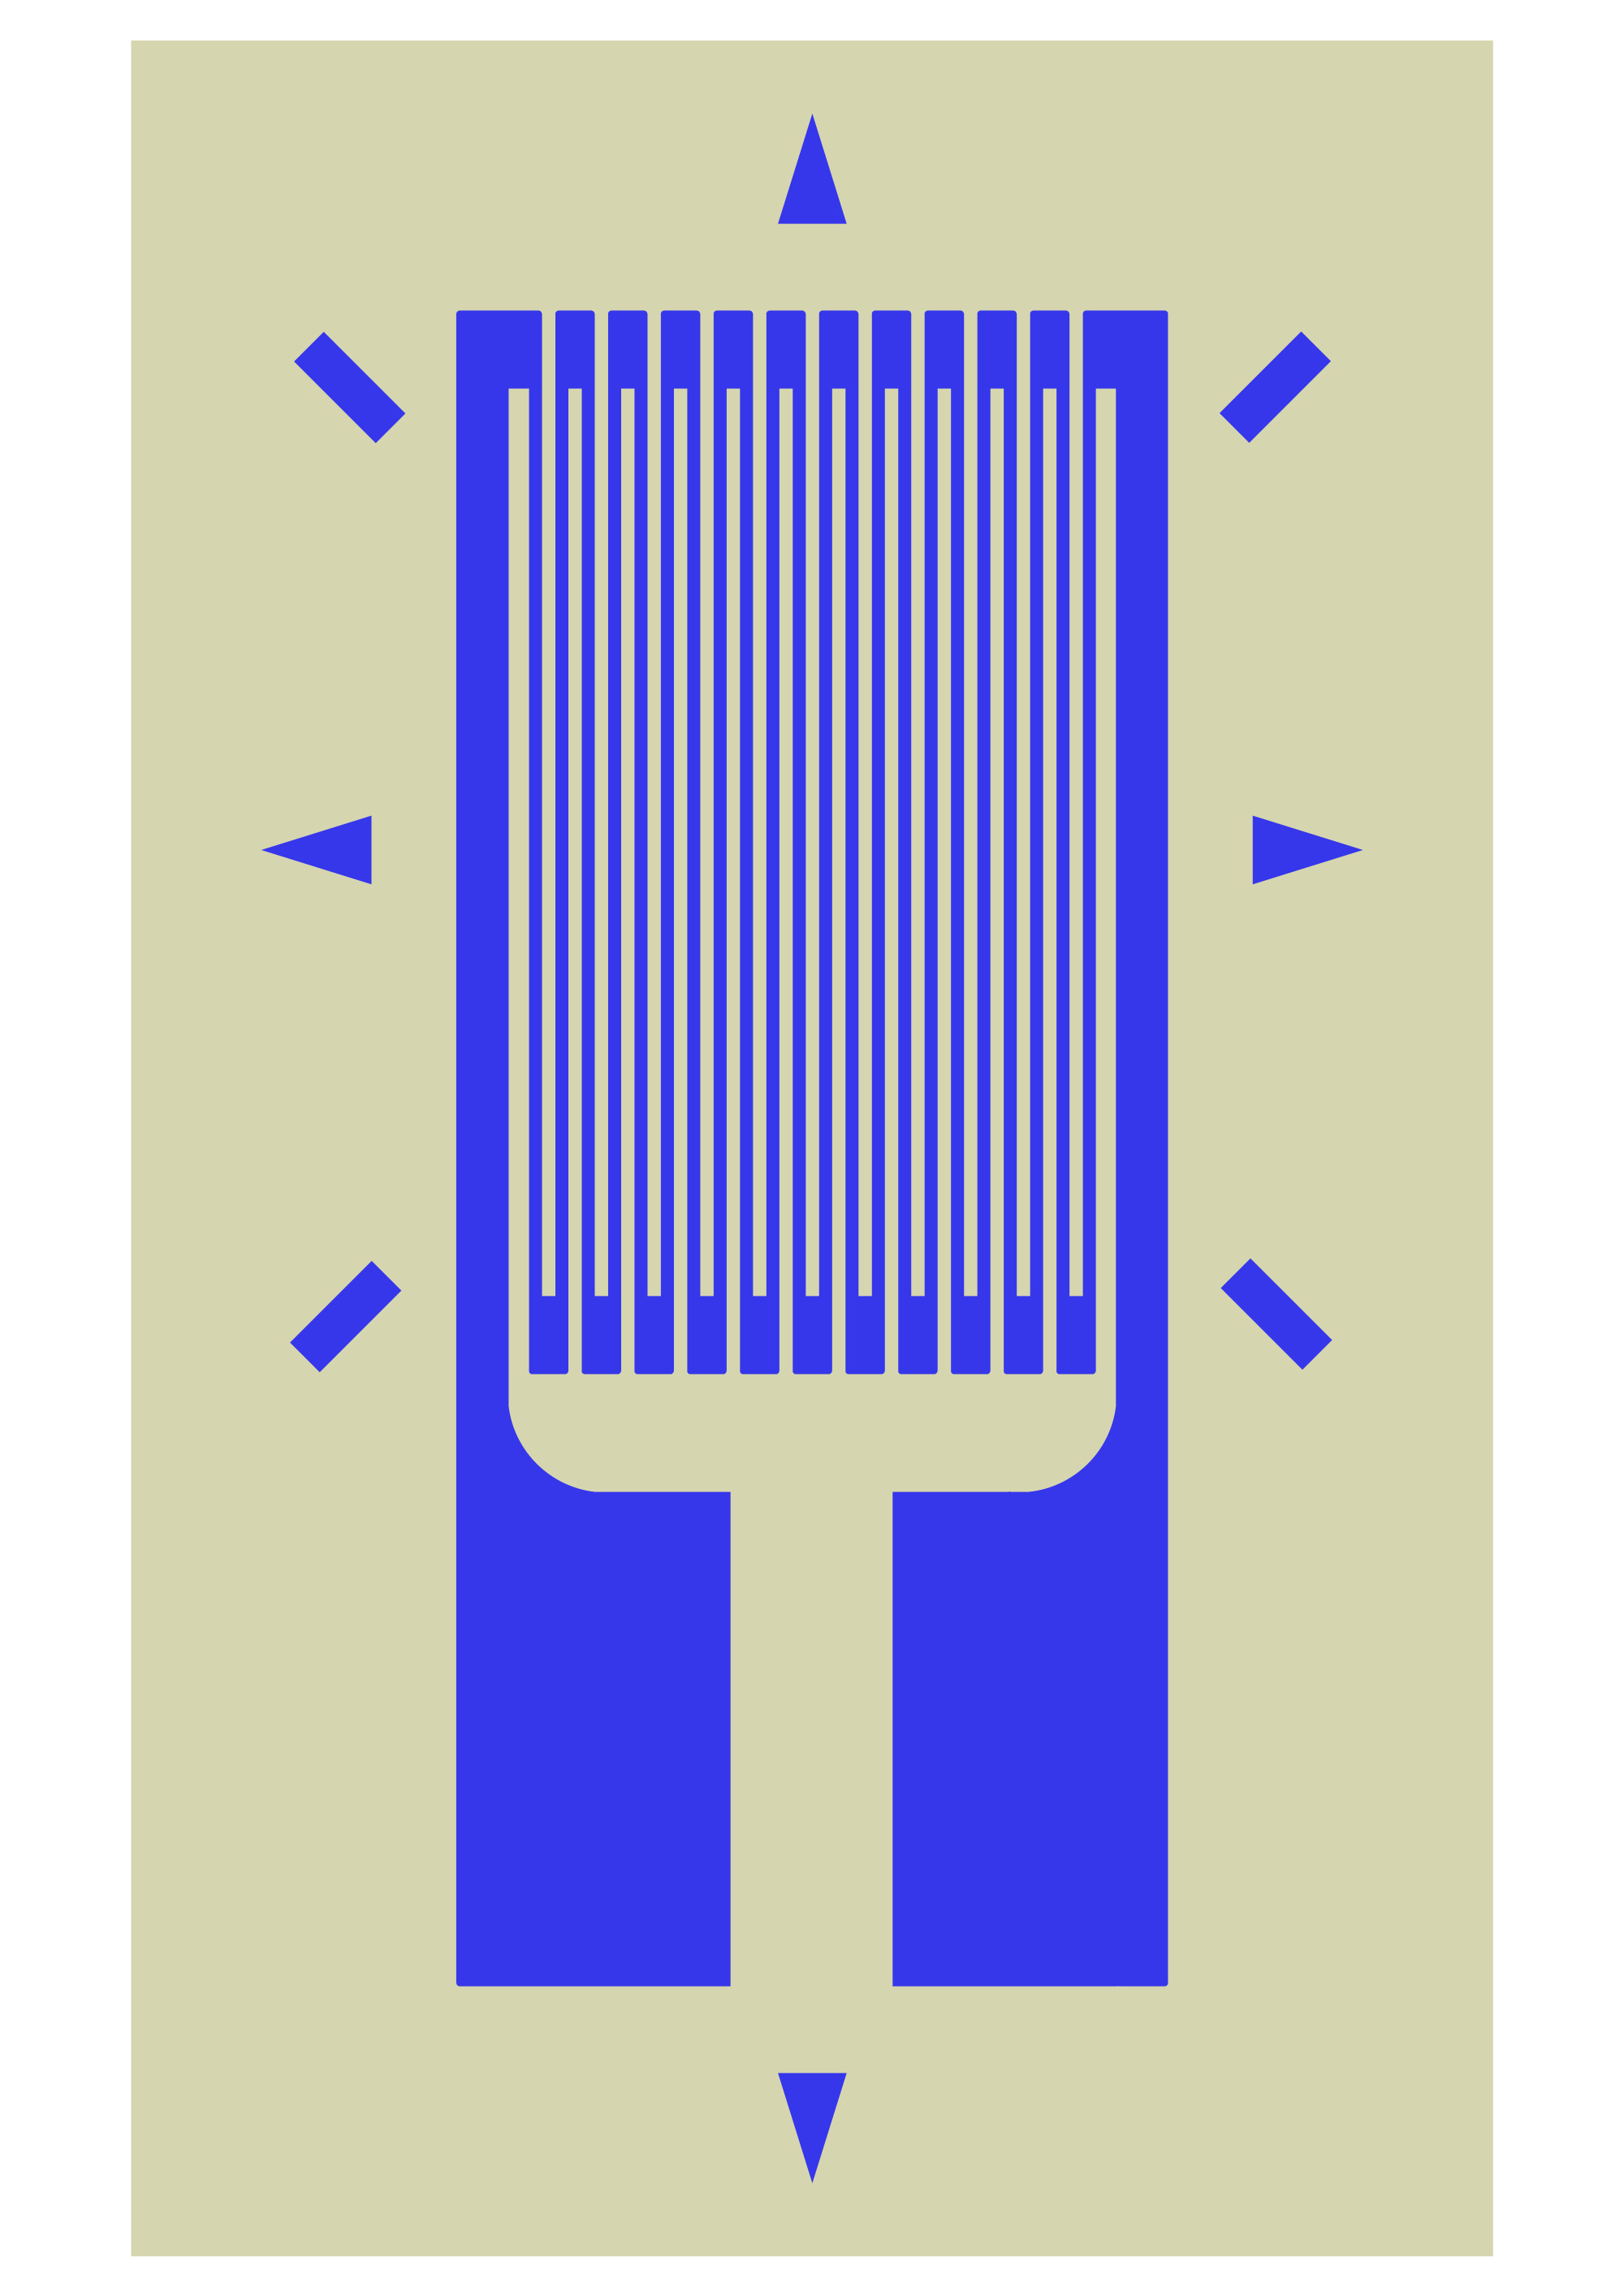
\includegraphics[width=0.4\textwidth]{strain.png}}}
\caption{Schematic of a typical metallic foil strain gage.  (This image is by ``MADe'', is licensed under the CC BY-SA license and is available from \url{http://en.wikipedia.org/wiki/File:Strain_gauge.svg}) }
\label{f:strain}
\end{figure}


\section{Signal Conditioning: Wheatstone Bridge}
The strain gage is one of many sensors where the transduction is a conversion to a small change in resistance.  Directly measuring such a small resistance within a data acquisition system is challenging.  It would be preferable if the input to our analog to digital converter was a voltage indicating the value of the physical quantity we are attempting to measure.  Enter the Wheatstone bridge.  This simple circuit is sketched in Figure~\ref{f:bridge}.  This particular implementation illustrates a ``quarter-bridge'' circuit, where the sensor is represented by the resistor value $R_x$.

\begin{figure}[hbt!]
\centerline{
{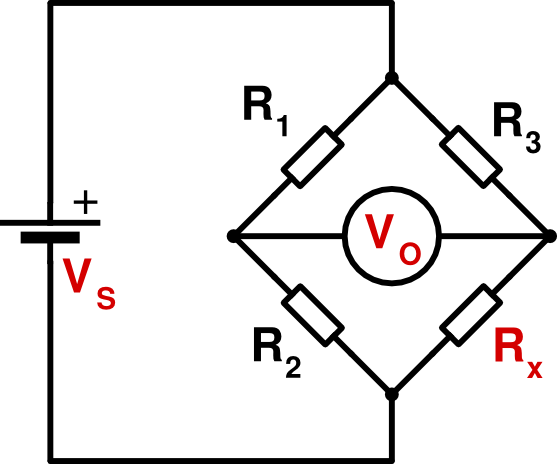
\includegraphics[width=0.5\textwidth]{Wheatstonebridge2.png}}}
\caption{ Wheatstone bridge circuit.  Excitation voltage is $V_s$, the strain gage (variable resistance) is $R_x$ and the output voltage is $V_o$. (This image an adaptation of the image by ``Zedh'', is licensed under the CC BY-SA license and is available from \url{http://en.wikipedia.org/wiki/File:Wheatstonebridge.svg}) }
\label{f:bridge}
\end{figure}

To get started, consider if the bridge is perfectly ``balanced'' which requires all the resistance values ($R_1$, $R_2$, $R_3$ and $R_x$) to be equivalent.  The \gls{bridge excitation voltage} ($V_S$) is applied as shown (e.g., $V_s=\unit[10]{V}$).  (The excitation voltage could also be called the supply voltage.) The output of the bridge circuit is $V_o$.  Given this scenario, with the bridge in a balanced state, what is the output voltage?  Hopefully it makes conceptual sense that this voltage would be zero.  Since the all the resistors are of the same value the voltage drop across each resistor would be equivalent.

When the value of one leg of the bridge changes, say when a strain induces a change in resistance of $R_x$, then the bridge us unbalanced and the output voltage is non-zero.  We won't do the circuit analysis here (there are plenty of examples online if you are interested), and instead we'll just present the result:
\begin{equation}\label{e:bridge}
V_o = V_s \left( \frac{\delta R_x/R_x}{4+2(\delta R_x/R_x)} \right) \approx \frac{\delta R_x/R_x}{4}.
\end{equation}
This expression quantifies how a change in resistance of one leg of a quarter-bridge circuit is converted into a corresponding output voltage.  Notice the sensitivity of the bridge circuit is a function of of the excitation voltage ($V_s$).  So, the larger the excitation the larger the output voltage, for an equivalent change in resistance.  (Of course the larger the supply voltage the larger the current flowing through the bridge which results in unnecessary heating which then causes other problems.)

There are other implementations of the Wheatstone bridge such as half-bridge and full-bridge configurations; we'll stick with the quarter-bridge for now.

\section{Strain Gage Data Acquisition}
\begin{figure}[hbt!]
\centering
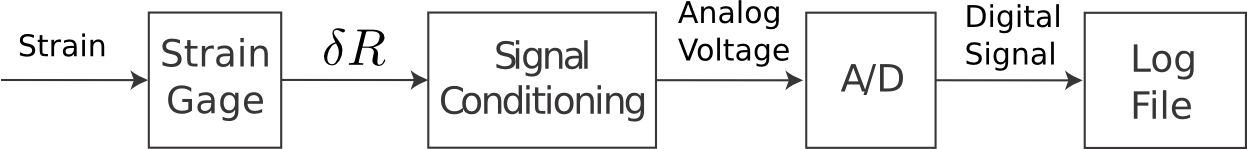
\includegraphics[width=\FigWidth\textwidth]{strain_daq.png}
\caption{A data acquisition including a strain gage and Wheatstone bridge.  See Figure~\ref{f:daq} for the general DAQ layout.}
\label{f:straindaq}
\end{figure}

By putting these components together we can build a complete data acquisition system for measuring strain as illustrated in Figure~\ref{f:straindaq}. To describe the mathematical relationship between physical strain and the analog voltage measured by the A/D we combine (\ref{e:gage}) and (\ref{e:bridge}) to generate the expression
\begin{equation} \label{e:gagebridge}
V_o \approx V_s\left( \frac{(\mathrm{GF})\epsilon}{4} \right).
\end{equation}

\section{Exercises}
\begin{ex}
Using (\ref{e:eps}) and (\ref{e:gagebridge}) derive a mathematical model (an equation) that predicts the voltage output of the Wheatstone bridge ($V_o$) as a function of the applied load at the free end of the beam.
\end{ex}
\ifsolutions
\begin{soln}
\[
V_o \approx V_s\left( \frac{\mathrm{GF}}{4} \right) \left(\frac{F(x-l)(h/2)}{EI}\right)
\]
\end{soln}
\fi
























